\section{Introduktion}

\begin{frame}{Introduktion}
  \begin{columns}[T]
    % Venstre kolonne (55% af bredden)
    \column{0.55\textwidth}
    \hspace*{1cm}
    \begin{minipage}{0.85\textwidth}
      \small
      \setlength{\parskip}{0.1cm} % Reduceret linjeafstand
      \RaggedRight
      \textbf{\large Aleksander Sonder} \par
      \vspace{0.05cm} % Minimal luft før sektioner
      \textbf{Jagterfaring} \par
      Jagttegn siden 1997 \par
      Jagttegnslærer \par
      Skydeinstruktør \par
      Riffel og haglgevær \par
      Hundefører \par
      \vspace{0.05cm} % Minimal luft før sektioner
      \textbf{Privat} \par
      Familiefar \par
      \vspace{0.05cm}
      \textbf{Professionelt} \par
      Selvstændig, bestyrelse mm \par
      \vspace{0.05cm}
      \textbf{Uddannelse} \par
      DTU, RUC mm \par
    \end{minipage}
    
    % Højre kolonne (45% af bredden)
    \column{0.45\textwidth}
    \centering
    \vspace*{0.4cm} % Lidt mindre vertikal plads øverst
    \fbox{
      
\includegraphics[width=0.7\textwidth]{Billeder/Andet/AKSS.jpg}
    }
    \vspace*{0.2cm} % Mindre plads under billedet
  \end{columns}
\end{frame}

\begin{frame}{Lidt om jer?}
  \begin{columns}[T]
    % Venstre kolonne (55% af bredden) – spørgsmål med bullets
    \column{0.55\textwidth}
    \hspace*{1cm}
    \begin{minipage}{0.85\textwidth}
      \small
      \setlength{\parskip}{0.1cm}
      \RaggedRight
      \begin{itemize}
        \item \large Navn?
        \item \large Hvorfor vil du tage jagttegn?
        \item \large Har du været med på jagt?
        \item \large Har du prøvet at skyde?
      \end{itemize}
    \end{minipage}
    
    % Højre kolonne (45% af bredden) – ikon
    \column{0.45\textwidth}
    \centering
    \vspace*{0.4cm} % Justerer lodret placering
    
\includegraphics[width=0.50\textwidth]{Billeder/Andet/target-audience.png}
  \end{columns}
\end{frame}

\begin{frame}{Formalia}
  \vspace{1em}
  \begin{columns}[T]
    \column{0.05\textwidth}
    \column{0.9\textwidth}
    \setlength{\parskip}{0.4em}
    \small
    \RaggedRight

    \textbf{JægerID:} \\
    \url{https://sgavmst.dk/natur-og-jagt/jagttegn/jagttegnsaspirant} \par

    \vspace{0.5em}
    \textbf{Simulerede teoriprøver:} \\
    \url{https://osjagttegn.dk/} (gratis)\\
    \url{https://jagtproeven.dk/} (100  kr) \par

    \vspace{0.5em}
    \textbf{Google Drive (præsentationer mm):} \\
    \url{https://drive.google.com/drive/folders/1iLtHqLLlpJ-f5kI5OEOSgUxoz1dal9t4?usp=sharing } \par

    \vspace{0.5em}
    \textbf{WhatsApp (chat/feedback):} \\
    \url{https://chat.whatsapp.com/BMfd13gMv2RL8rK3jt25jy} \par

    \column{0.05\textwidth}
  \end{columns}
\end{frame}

\begin{frame}{Våbenhåndtering og sikkerhedsregler}
  \vspace{1em}
  \begin{columns}[c] % c = center vertically
    \column{0.05\textwidth} % Venstre margin (kan fjernes eller justeres)

    \column{0.7\textwidth} % Midten: Bullets
    \small
    \raggedright

    \begin{itemize}
      \itemsep0.6em % Justér afstand mellem bullets
      \item Brug alle muligheder for at øve våbenhåndtering (tørtræning) med haglgevær.
      \item Våben må \alert{ikke} forlade kursuslokalet/gangen.
      \item Våben må \alert{kun} håndteres i Aleksanders nærvær.
      \item Brug \alert{altid} klikpatroner.
    \end{itemize}

    \column{0.25\textwidth} % Højre: Ikon (størrelsen tilpasses her)
    \centering
    \vspace{0pt} % hjælper med vertikal centring i nogle temaer
    
\includegraphics[width=0.8\linewidth]{Billeder/Andet/shotgun.png}

  \end{columns}
\end{frame}

\begin{frame}{Materiale}
  \vspace{1em}
  \begin{columns}[T]
    \column{0.05\textwidth}

    \column{0.9\textwidth}
    \setlength{\parskip}{0.4em}
    \small
    \RaggedRight

    \textbf{Jagttegn – 6. udgave:} \\
    Niels Søndergård, ISBN 978-87-93976-28-3 \\
    \url{https://netbutikken.seges.dk/index.php/jagt/jagttegn-541.html} \par

    E-bog/PDF version: \\
    \url{https://jagtproeven.dk/materialer/boger/} \par

    \vspace{0.5em}
    \textbf{Supplerende:} \\[0.2em]
    Lovsamling til jægeren 2024–2025 \\
    \url{https://netbutikken.seges.dk/index.php/jagt/lovsamling-til-jaegeren-2024-25.html} \par

    Wildcards \\
    \url{https://netbutikken.seges.dk/index.php/jagt/wildcards.html} \par

    Fuglekort \\
    \url{https://www.fuglekort.com/} \par

    \column{0.05\textwidth}
  \end{columns}
\end{frame}

\begin{frame}{Teoriemner}
\begin{itemize}
    \item Artsbestemmelse
    \item Vildtforvaltning
    \item Jagtvåben og ammunition
    \item Jagtlovgivning
    \item Håndtering af nedlagt vildt
    \item Jagtetik og -etikette
    \item Jagtteknik og -ledelse
    \item Skudafgivelse med forskellige våben
\end{itemize}
\end{frame}

\begin{frame}{Lektionsplan}
  \vspace{1em}
  \begin{columns}[T]
    \column{0.05\textwidth}

    \column{0.9\textwidth}
    \setlength{\parskip}{0.4em}
    \small
    \RaggedRight

    \textbf{Lektionsplan}

    \column{0.05\textwidth}
  \end{columns}
\end{frame}


\begin{frame}
  \vspace{3em}
  \begin{center}
    {\LARGE \textbf{Jagtprøven}}
  \end{center}
\end{frame}



\section{Jagtprøven}

\begin{frame}{Jagtprøven – teoretisk del}
  \vspace{0.8em}
  \begin{columns}[T]
    \column{0.05\textwidth}

    \column{0.9\textwidth}
    \setlength{\parskip}{0.4em}
    \footnotesize
    \RaggedRight

    Teoretisk prøve skal bestås \textbf{før} praktisk prøve kan aflægges \par

    40 spørgsmål – \textbf{maks. 4 fejl} \par

    30 min. uden hjælpemidler (\textbf{45 sek. pr. spørgsmål}) \par

    Multiple choice i forskellige variationer \par

    \vspace{0.3em}
    \textbf{Emner (antal spørgsmål):} \\
    Jagtlovgivning (13), Vildtkendskab (10), \\
    Vildtbiologi/jagt/vildtforvaltning (8), \\
    Jagtvåben/ammunition (3), \\
    Etik/jagtteknik/jagtledelse (3), \\
    Sikkerhed (3) \par

    \vspace{0.3em}
    \textbf{3 forsøg} \par

    \vspace{0.2em}
    \textit{Bestås teoriprøven, men dumpes den praktiske prøve, \\
    skal teoriprøven \textbf{ikke} aflægges igen inden for de 3 forsøg.} \par

    \column{0.05\textwidth}
  \end{columns}
\end{frame}

\begin{frame}{Jagtprøven – praktisk del}
  \vspace{1em}
  \begin{columns}[T]
    \column{0.05\textwidth}

    \column{0.9\textwidth}
    \setlength{\parskip}{0.5em}
    \small
    \RaggedRight

    Sikker håndtering af haglgevær \par

    Sikker forcering af forhindringer (hegn/grøft) \par

    6 afstandsbedømmelser til vildtfigurer (\textbf{maks. 1 fejl}) \par

    Sikker afgivelse af skud til lerduer (bagduer) – \\
    \textit{ikke et krav at ramme!} \par

    \vspace{0.4em}
    \textbf{3 forsøg} \par

    \vspace{0.3em}
    \textit{Bestås praktisk prøve ikke, må teoriprøven \\
    \textbf{beholdes} inden for de 3 forsøg.} \par

    \column{0.05\textwidth}
  \end{columns}
\end{frame}

\begin{frame}{Praktisk prøve - visualisering}
    \centering
    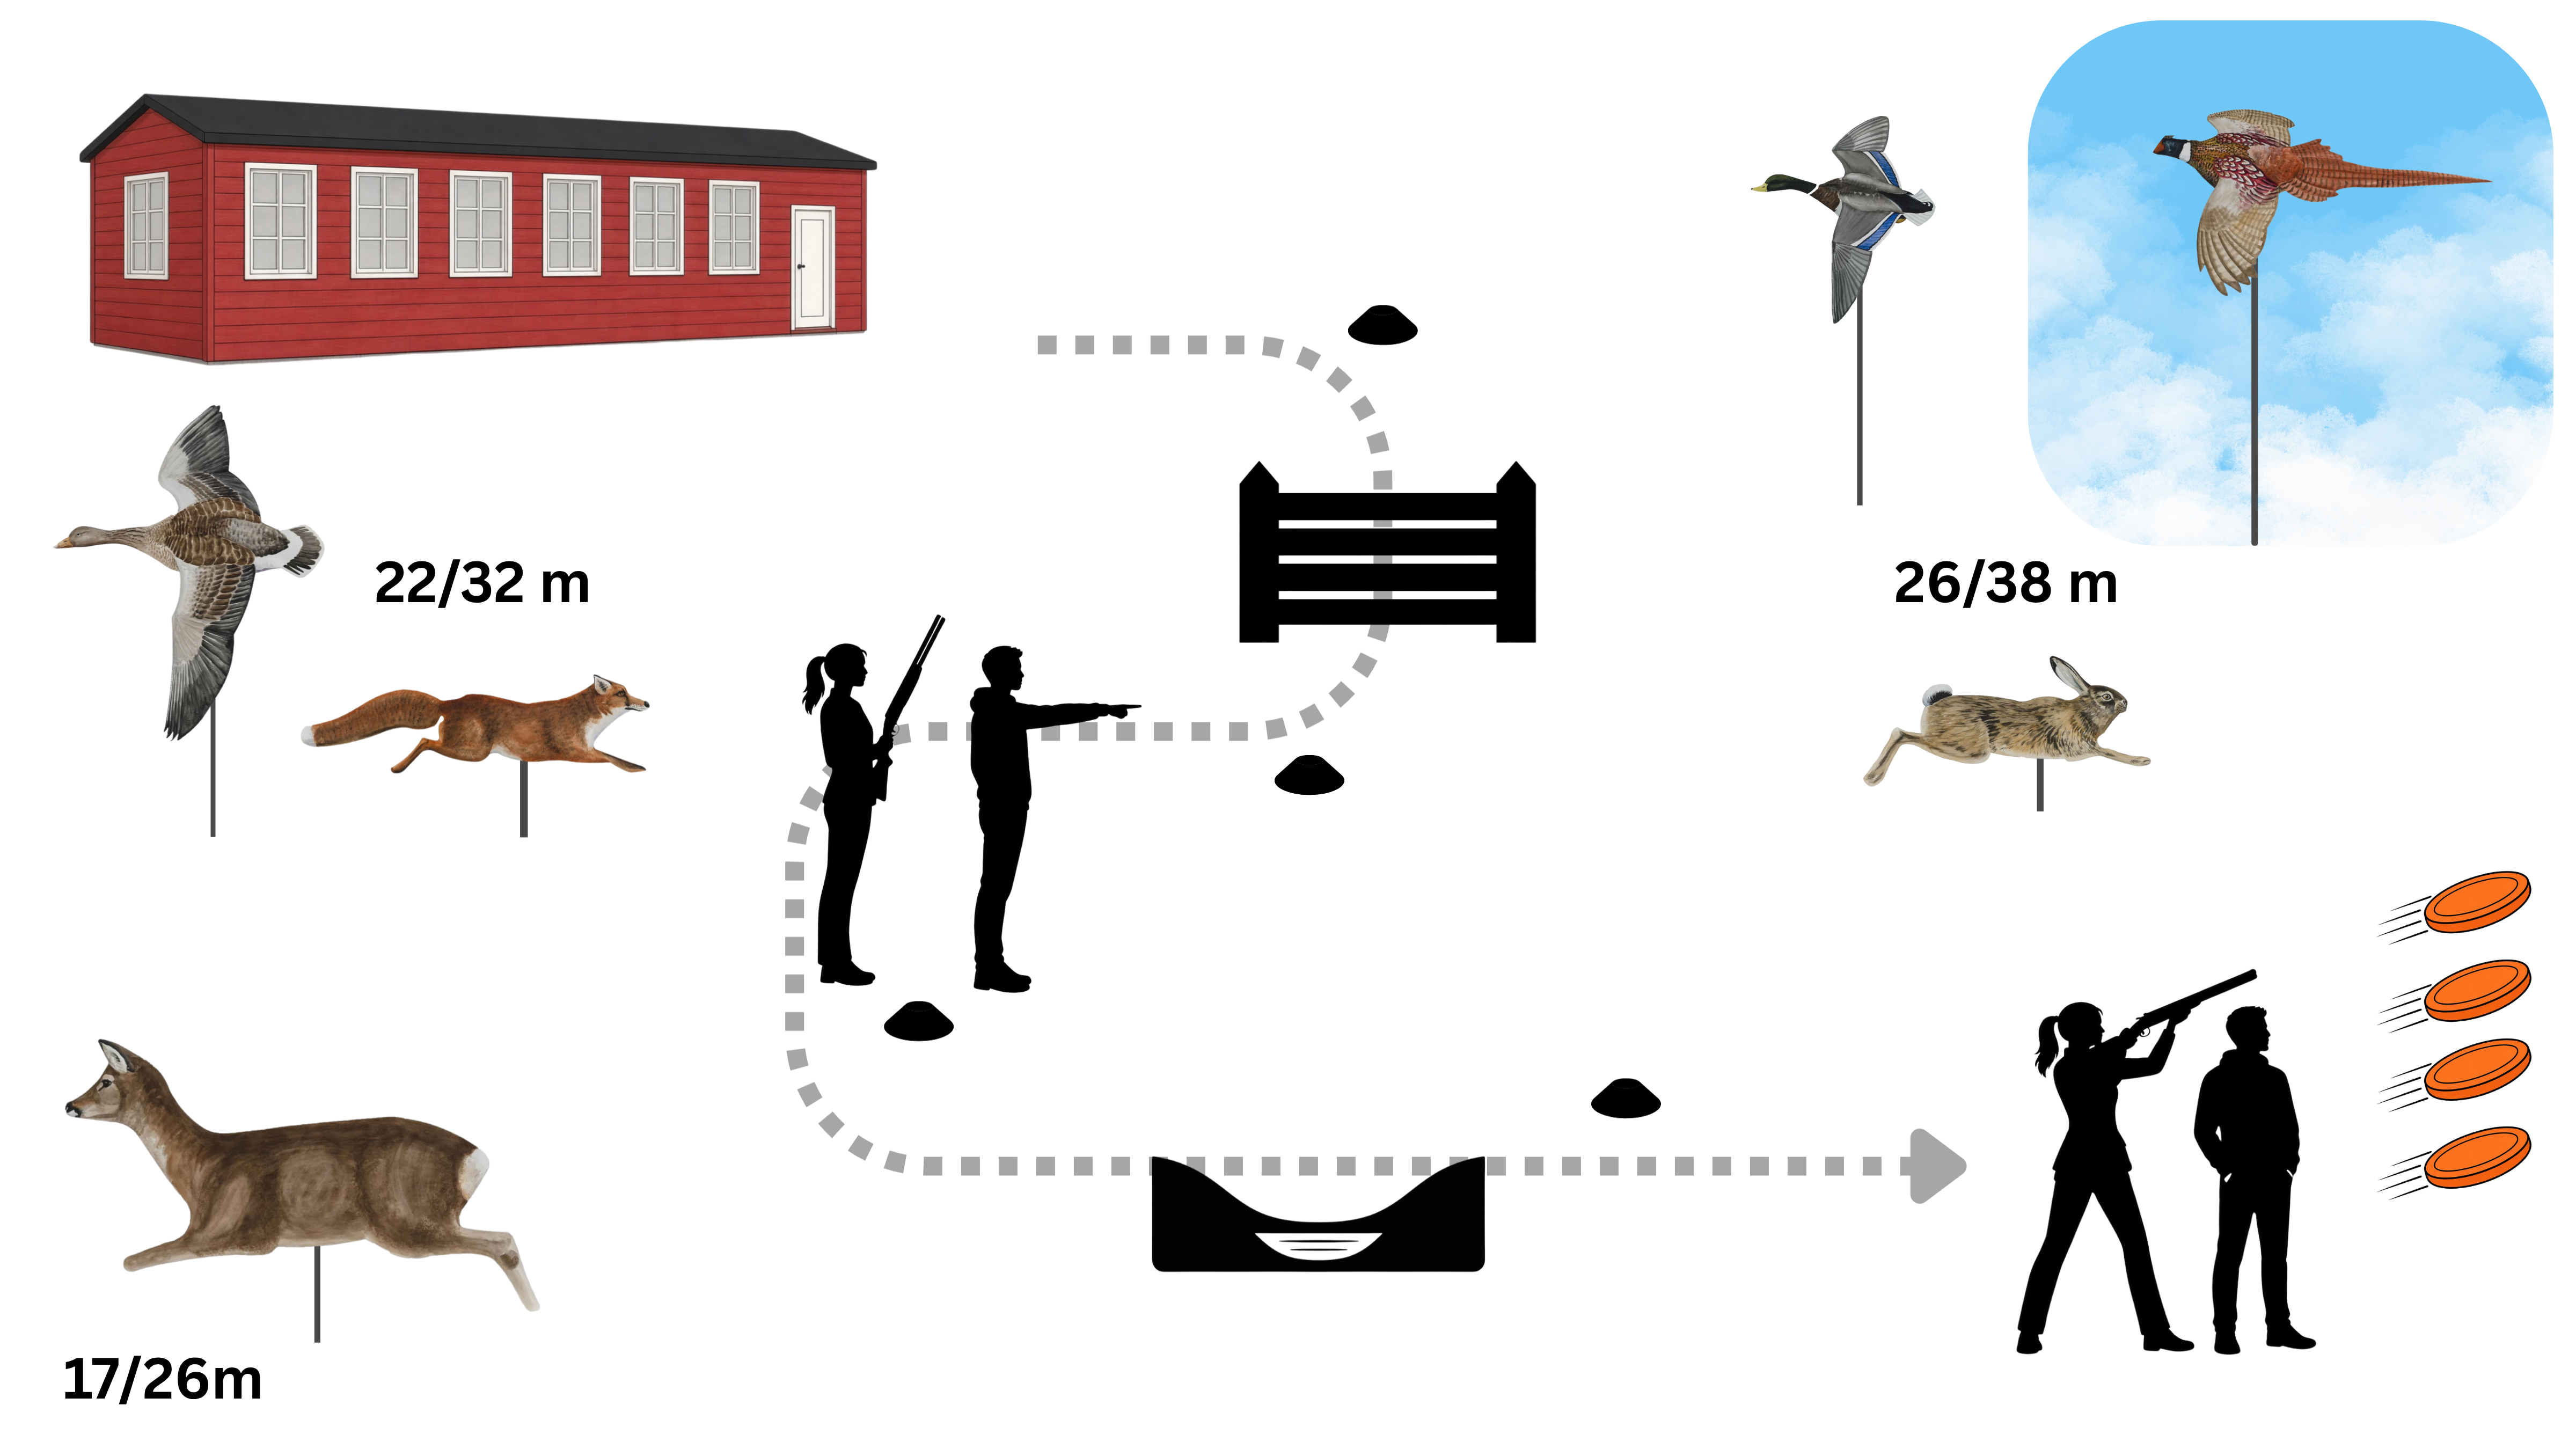
\includegraphics[width=0.85\textwidth]{Billeder/Andet/2638 m (1).png}
\end{frame}

\begin{frame}{Vejen til jagttegn}
\centering
\resizebox{0.85\textwidth}{!}{%
\begin{figure}[!ht]
\centering
\begin{circuitikz}
\tikzstyle{every node}=[font=\Large]

% Obligatorisk jagttegnskursus
\draw [rounded corners=7.8] (11.5,18.5) rectangle node {\Large Obligatorisk jagttegnskursus} (20.5,16.5);

% Jagttegnsprøven
\draw [rounded corners=7.8] (13,15) rectangle node {\Large Jagttegnsprøven} (19,13.5);
\draw [->, >=Stealth] (16,16.5) -- (16,15);

% Jagttegn
\draw [rounded corners=7.8] (13,12) rectangle node {\Large Jagttegn} (19,10.5);
\draw [->, >=Stealth] (16,13.5) -- (16,12);

% De fire prøver
\draw [rounded corners=7.8] (2.5,8.5) rectangle node {\Large Haglskydeprøve} (8.5,7);
\draw [rounded corners=7.8] (9.5,8.5) rectangle node {\Large Riffelprøve} (15.5,7);
\draw [rounded corners=7.8] (16.5,8.5) rectangle node {\Large Bueprøve} (22.5,7);
\draw [rounded corners=7.8] (23.5,8.5) rectangle node {\Large Falkonerprøve} (29.5,7);

\draw [->, >=Stealth] (16,10.5) -- (5.5,8.5);
\draw [->, >=Stealth] (16,10.5) -- (12.5,8.5);
\draw [->, >=Stealth] (16,10.5) -- (19.5,8.5);
\draw [->, >=Stealth] (16,10.5) -- (26.5,8.5);

% Påtegning
\draw [rounded corners=7.8] (13,5) rectangle node {\Large Påtegning til jagttegn} (19,3.5);
\draw [->, >=Stealth] (5.5,7) -- (16,5);
\draw [->, >=Stealth] (12.5,7) -- (16,5);
\draw [->, >=Stealth] (19.5,7) -- (16,5);
\draw [->, >=Stealth] (26.5,7) -- (16,5);

\end{circuitikz}
\end{figure}
}%
\end{frame}